%%%%LEZIONE 5 APRILE%%%%
Lezione del 05/04, ultima modifica 20/05, Andrea Gadotti
\\
In generale una statistica test si può descrivere come di seguito:\\
$$\bigg \{
\begin{array}{rl}
H_0: & \theta \in \Theta_0 \\
H_1: & \theta \in \Theta_1 \\
\end{array}
$$
\\
dove $\Theta$ è lo spazio dei possibili parametri della distribuzione e $\Theta = \Theta_0 \cup \Theta_1$.\\
Quello che vogliamo trovare è la regola di partizionamento che divida lo spazio dei campioni $C$ in $C_0$ e $C_1$ in funzione di $\alpha$ (deciso da noi). Per farlo imponiamo la condizione $\alpha = P(\underline{x} \in C \mid \theta \in \Theta_0)$. Vediamo ora un esempio con il lancio di una moneta:\\
\\
\noindent \textbf{Esempio} Consideriamo il campione casuale $(X_1,...,X_n)$ dove $X_i = 0$ con probabilità $p$ e $X_i = 1$ con probabilità $1-p$. Facciamo le nostre ipotesi:\\
$$\bigg \{
\begin{array}{rl}
H_0: & p \leq 1/2 \\
H_1: & p > 1/2 \\
\end{array}
$$
\\
Prediamo ora come regola di decisione $\frac{S}{n}=\frac{\sum X_i}{n}$. Deciso un $\alpha$ a nostra discrezione, imponiamo l'equazione in $k$:
$$ \alpha = P(S>k \mid p \leq 1/2) \; (= P(S>k \mid H_0 \text{ vera}))$$
A questo punto risolvendo l'equazione troveremo il $k$ per il quale rifiuteremo $H_0$ se $S>k$.\\
\\
\noindent \textbf{Esempio} Sia $(X_1,...,X_n)$ un campione casuale con $X_i \sim b(1,p)$ e sia\\
$$\bigg \{
\begin{array}{rl}
H_0: & p=p_0 \\
H_1: & p<p_0 \\
\end{array}
$$
\\
Sulla base dell'informazione circa $p$ contenuta in $(X_1,...,X_n)$ vogliamo sottoporre a verifica il sistema di ipotesi in questione. Procediamo in questo ordine:\\
\begin{enumerate}
\item [(a)] Prendiamo $S:=\sum X_i \sim b(n,p)$, che è di fatto il numero di successi. Sotto $H_0$ abbiamo che $S \sim b(n,p_0)$.
\item [(b)] Scegliamo una regola di decisione (usando anche la distribuzione -nota- di $S$ sotto $H_0$). Ovvero, individuiamo la \textit{regione di rifiuto del test}. A questo punto vorremo rifiutare $H_0$ a favore di $H_1$ quando $S \leq k$, dove $k$ è l'incognita che troveremo nel punto (c).
\item [(c)] Scelto il nostro $\alpha$, si ha che il valore di $k$ deve essere tale per cui 
			$$\alpha = P(S \leq k \mid p=p_0) = \displaystyle \sum_{s=0}^k \binom{n}{s} p_0^s (1-p_0)^{n-s}$$
A questo punto, essendo $\alpha$ fissato, abbiamo un'equazione in $k$ che risolta ci restituisce il suo valore.
\end{enumerate}
\textbf{Esempio particolare} Nella situazione generale sopra descritta prendiamo un caso particolare con $n=20$ e $p_0=0,7$. Decidiamo $\alpha = 0.15$. L'equazione diventa: $0,15 = \sum_{s=0}^k \binom{20}{s} 0,7^s 0,3^{20-s}$. Osserviamo che il valore di $P(S \leq k \mid p=0,7)$ per $k=11$ risulta $0,1133$, mentre per $k=12$ è $0,2277$. Quindi il nostro $k$ è compreso tra 11 e 12. In conclusione, se il nostro test dovesse presentare 12 (o più) successi, allora non rifiuteremmo $H_0$. In caso contrario scarteremmo $H_0$ a favore di $H_1$.

\begin{definizione} Sia $\beta := P(\underline{x} \in C_0 \mid \theta \in \Theta_1)$, ovvero $\beta$ è la probabilità (fissato $\alpha$) di commettere un errore di II specie. Chiamiamo \textit{potenza del test} il valore $\gamma := 1-\beta$. Un test risulta ottimale quando la sua potenza è massima. Notiamo che possiamo definire una \textit{funzione di potenza} $\gamma(t) := 1-\beta(t)$
\end{definizione}
\begin{oss} Prendendo di nuovo in considerazione l'esempio precedente sul campione casuale normale, è chiaro che una volta fissato $\alpha$, ovvero $c$, minore è $\mu_1$, più piccola è l'area sottesa dalla coda della relativa normale, ovvero $\beta$.
\end{oss}
\noindent \textbf{Esempio} Prendendo di nuovo in considerazione l'esempio precedente sulla bernoulliana, abbiamo che 
			$$\gamma(p) = P(S \leq k \mid p<p_0) = \displaystyle \sum_{s=0}^k \binom{n}{s} p^s (1-p)^{n-s}$$
Di seguito possiamo osservare il grafico della funzione:\\
\\
\begin{center}
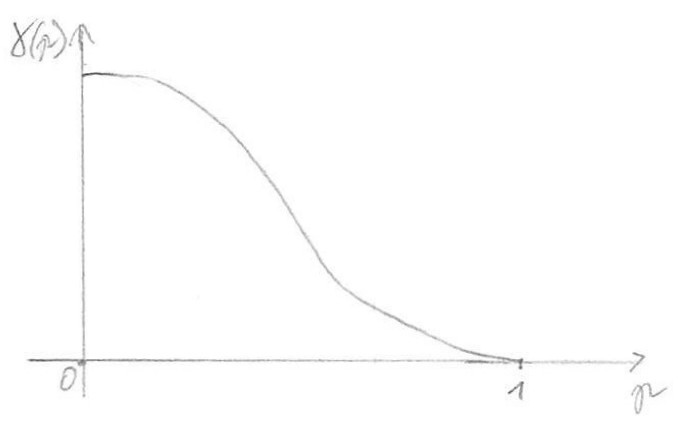
\includegraphics [width=12cm] {immagini/grafico_3.jpg}
\end{center}
\textbf{Osservazione} Il test in merito al precedente sistema di ipotesi relative a $p$ è un \textit{test esatto}, perché poggia sulla distribuzione \textit{esatta} di $S$ ($S \sim b(n,p)$). Questo però non accade sempre, e quindi talvolta è necessario ricorrere alla teoria asintotica e dei test approssimati.\\


\subsection{Esempi di statistiche test (generali e particolari)}

\textbf{Test per la media di una popolazione qualsiasi} Supponiamo di avere un campione casuale $(X_1,...,X_n)$ proveniente da una distribuzione \underline{non} nota di media $\mu$ e varianza $\sigma^2$ (finita) \underline{non} note.\\
Le nostre ipotesi sono 
$$\bigg \{
\begin{array}{rl}
H_0: & \mu=\mu_0 \\
H_1: & \mu>\mu_0 \\
\end{array}
$$
Decidiamo di ''condensare'' l'informazione presente nel campione circa $\mu$ e $\sigma^2$ tramite $\overline{X}_n$ e $S_n^2$ (che ricordiamo essere stimatori non distorti e consistenti), sapendo che $\overline{X}_n \stackrel{P}{\rightarrow} \mu$ e $S_n^2 \stackrel{P}{\rightarrow} \sigma^2$.\\
A questo punto, la nostra regola di decisione consisterà nel rifiutare $H_0$ a favore di $H_1$ se $\overline{X}_n$ è molto più grande di $\mu_0$.\\
Noi sappiamo che $\overline{X}_n \stackrel{a}{\sim} N \left( \mu, \frac{S_n^2}{n}\right)$, ovvero $\frac{\overline{X}_n-\mu}{S_n/\sqrt{n}} \stackrel{D}{\rightarrow} N(0,1) =: Z$\\
Usando questo risultato possiamo individuare la regione critica del test di livello $\alpha$ fissato. Imponiamo la seguente uguaglianza:

\begin{eqnarray}
\alpha 	&=& P(\overline{x} \in C \mid \mu=\mu_0) = P(\overline{X}_n \geq k \mid \mu=\mu_0) \nonumber \\
		&=& P \left( \frac{\overline{X}_n-\mu}{S_n/\sqrt{n}} \geq \frac{\overline{k}-\mu}{S_n/\sqrt{n}} \mid \mu=\mu_0 \right) \nonumber \\
		&=& P \left( \frac{\overline{X}_n-\mu_0}{S_n/\sqrt{n}} \geq \frac{\overline{k}-\mu_0}{S_n/\sqrt{n}} \right) = P(Z \geq z_{\alpha}) \nonumber
\end{eqnarray}

Dove $z_{\alpha}$ è il valore da cercare sulle tavole relative alla distribuzione normale in funzione dell'$\alpha$ scelto. Nota: l'ultima uguaglianza è in realtà un'approssimazione che è tanto più corretta quanto più grande è $n$.\\
In definitiva, abbiamo che $C = \lbrace \underline{x} \in \varkappa \; : \; \frac{\overline{X}_n-\mu_0}{S_n/\sqrt{n}} \geq z_{\alpha} \rbrace = \lbrace \underline{x} \in \varkappa \; : \; \overline{X}_n \geq \mu_0 + z_{\alpha} \frac{S}{\sqrt{n}} \rbrace$\\

Possiamo anche considerare la \textit{funzione di potenza approssimata}:

\begin{eqnarray}
\gamma(\mu) = 1- \beta(\mu) 	&=& P(\overline{X}_n \geq \mu_0 + z_{\alpha} \sigma / \sqrt{n} \mid \mu > \mu_0) \nonumber \\
							&=& P \left(\frac{\overline{X}_n-\mu}{\sigma / \sqrt{n}} \geq \frac{\mu_0 + z_{\alpha} \sigma / \sqrt{n} - \mu}{\sigma / \sqrt{n}} \right) \nonumber \\
							&=& 1-P \left( Z \geq z_{\alpha} + \frac{\sqrt{n}(\mu_0 - \mu)}{\sigma} \right) \nonumber \\
							&=& 1-\Phi \left( z_{\alpha} + \frac{\sqrt{n}(\mu_0 - \mu)}{\sigma} \right) \nonumber
\end{eqnarray}

dove $\Phi$ è la funzione di ripartizione di $N(0,1)$.\\
Notiamo che il valore di $\gamma(\mu)$ tende a 1 per $n \rightarrow \infty$. Intuitivamente, questo è esattamente ciò che ci aspettiamo, in quanto più è grande $\mu$, più esso è distante dal nostro $\mu_0$, e di conseguenza è lecito aspettarsi che la probabilità che un campione abbia media vicina a $\mu$ sarà bassa, ovvero la potenza del test è elevata.\\
È chiaro quindi che una funzione di potenza è tanto migliore quanto più il suo grafico sta vicino alla retta $y=1$.\\
\\
\textbf{Esempio} In riferimento al caso generale appena trattato, supponiamo di avere $\mu_0=12$, $\overline{X}_n=14,3$, $S_n^2=22,5$, $n=50$. Se fissiamo $\alpha=0,05$, usando le tavole per la distribuzione normale $N(0,1)$ troviamo $z_{\alpha}=1,645$. Ne segue che $k=12+1,645\sqrt{22,5/50}$, che è minore di $14,3$. Concludiamo quindi rifiutando $H_0$.\\
\\
\textbf{Esempio di test esatto con t di Student} Abbiamo $(X_1,...,X_n)$ campione casuale da $N(\mu,\sigma^2)$ con $\mu$ e $\sigma^2$ non noti. Le nostre ipotesi sono:
$$\bigg \{
\begin{array}{rl}
H_0: & \mu=\mu_0 \\
H_1: & \mu>\mu_0 \\
\end{array}
$$
Sappiamo che $\overline{X}_n \stackrel{H_0}{\sim} N(\mu_0,\sigma^2/n)$ e quindi:
$$T:= \frac{\overline{X}_n - \mu_0}{S_n / \sqrt{n}} = \frac{\overline{X}_n - \mu_0}{\sigma / \sqrt{n}} \frac{1}{\sqrt{S_n^2 / \sigma^2}} \sim \frac{Z}{S_n / \sqrt{n}} \sim t_{n-1}$$
(vedi pag. 17 e pag. 12)\\
A questo punto, possiamo trovare il nostro valore critico $k$ usando le tavole della distribuzione $t_{n-1}$.\\
Notiamo che quello appena mostrato è un \textit{test esatto}, in quanto non si basa su un'approssimazione dello stimatore per valori elevati di $n$ (usando ad esempio il TLC), bensì usa la sua distribuzione reale (in questo caso la distribuzione $t_{n-1}$).